\documentclass[10pt]{article}
%fleqn
\usepackage{graphicx}
\usepackage{wrapfig}
\usepackage{url}
\usepackage{wrapfig}
\usepackage{color}
\usepackage{marvosym}
\usepackage{enumerate}
\usepackage{subfigure}
\usepackage{tikz}
\usepackage{amsmath}
\usepackage{amssymb}
\usepackage{hyperref} 

\usepackage{array}
\usepackage{calc}

\newlength\celldim
\newlength\fontheight
\newlength\extraheight
\newcounter{sqcolumns}

\newcolumntype{S}{
	@{}
	>{\centering \rule[-0.5\extraheight]{0pt}{\fontheight + \extraheight}%
		\begin{minipage}{\celldim}\centering}
		p{\celldim}
		<{\end{minipage}} 
	@{} }

\newcolumntype{Z}{ @{} >{\centering} p{\celldim} @{} }

\newenvironment{squarecells}[1]
{\setlength\celldim{4.5em}%
	\settoheight\fontheight{A}%
	\setlength\extraheight{\celldim - \fontheight}%
	\setcounter{sqcolumns}{#1 - 1}%
	\begin{tabular}{|S|*{\value{sqcolumns}}{Z|}}\hline}
	% squarecells tabular goes here
	{\end{tabular}}

\newcommand\nl{\tabularnewline\hline}

\oddsidemargin 0mm
\evensidemargin 5mm
\topmargin -20mm
\textheight 240mm
\textwidth 160mm

\newcommand{\vwi}{{\bf w}_i}

\pagestyle{myheadings} 
\markboth{}{Law of Large Graphs}

\title{Law of Large Graphs}
\author{}
\date{}

\begin{document}
	\large
	\maketitle
	\thispagestyle{headings}
	
	\vspace{-.5in}
	
	\section{Simulations}
	To demonstrate the previous results, we simulate random graphs from a SBM with parameters.
	\begin{equation*}
	B = \begin{bmatrix}
	.42 & .2 \\
	.2 & .7 
	\end{bmatrix}
	,\qquad \rho = \begin{bmatrix}
	.5 & .5
	\end{bmatrix}
	\end{equation*}
	
	From this model we sample $M$ Adjacency Matrices with $N$ vertices to calculate both $\bar{A}$ and $\hat{P}$.  With these estimators for $P$, we calculate the mean squared error of each block region in the model, and compare these with our predictions.
	
	\begin{figure}[!htb]
		\centering
		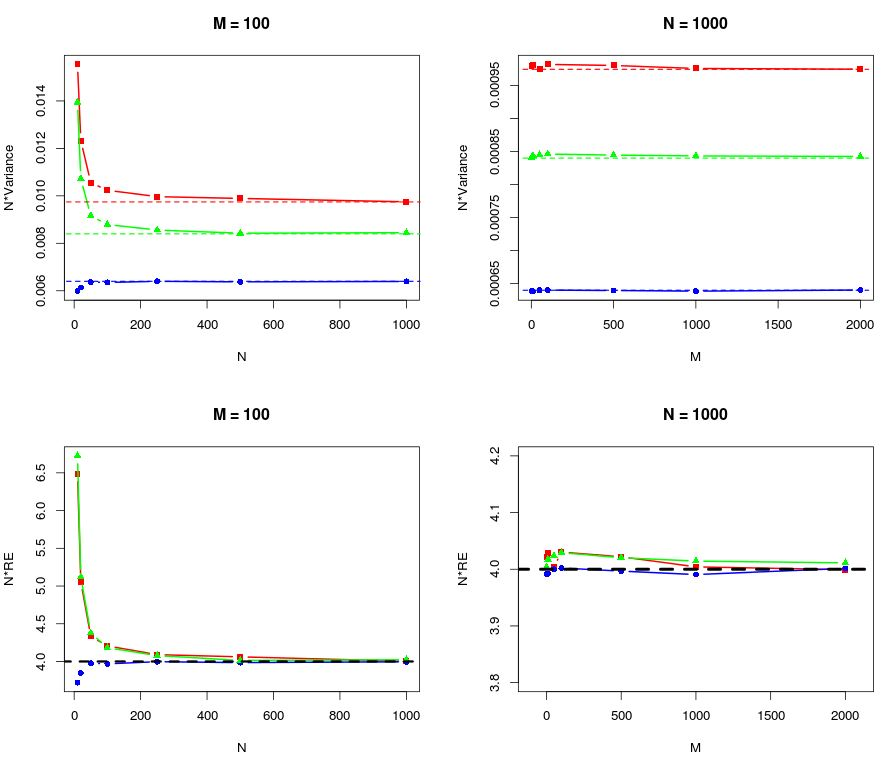
\includegraphics[width=16cm]{Var_RE.JPG}
		\caption{N*Variance$(\hat{P})$ and RE, dotted lines represent the predictions and each color represents unique values within the true $P \in \{.2,.42,.7\}$ }
		\label{fig:plot1}
	\end{figure}
	
	We now examine simulations where we vary the $\rho$ vector for the SBM with the following parameters:
	
		\begin{equation*}
		B = \begin{bmatrix}
		.42 & .2 \\
		.2 & .7 
		\end{bmatrix}
		,\qquad N = 500,\qquad M = 100
		\end{equation*}
	
	\begin{figure}[!htb]
		\centering
		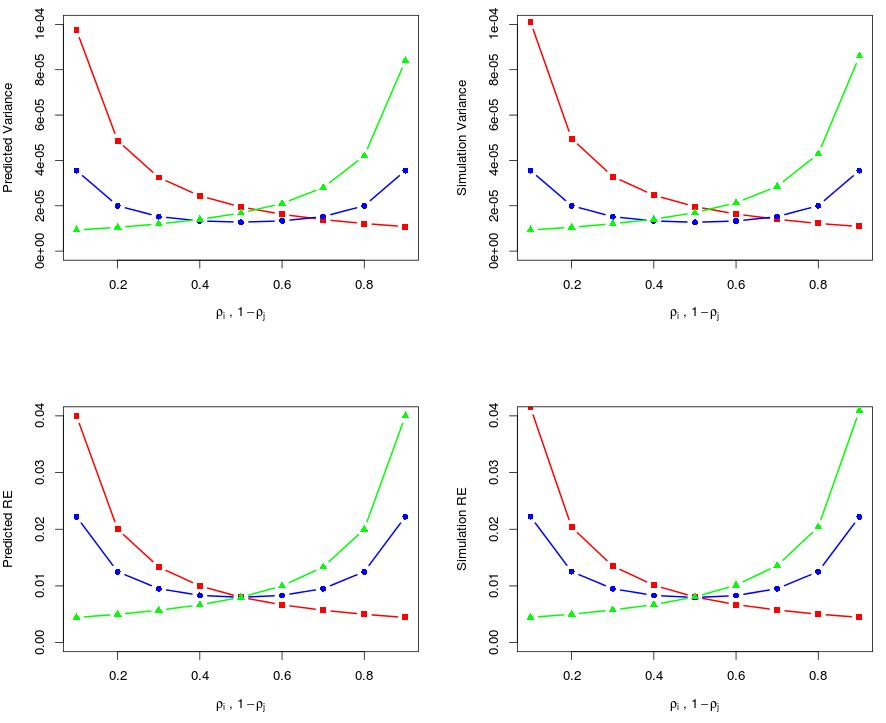
\includegraphics[width=16cm]{PI.JPG}
		\caption{N*Variance$(\hat{P})$ and RE, plots on the left are Predicted values corresponding to the right plot and each color represents unique values within the true $P \in \{.2,.42,.7\}$ }
		\label{fig:plot1}
	\end{figure}
	
	\paragraph{Cross-validation study with real data}
\end{document}